\documentclass[peerreview]{ieeesyscoin}
\usepackage{cite}
\usepackage{amsmath,amssymb,amsfonts}
\usepackage{algorithmic}
\usepackage{enumitem}
\usepackage{caption}
\usepackage{xcolor}
\usepackage{graphicx}
\usepackage{textcomp}
\usepackage{multirow}
\usepackage[switch]{lineno}
\def\BibTeX{{\rm B\kern-.05em{\sc i\kern-.025em b}\kern-.08em
    T\kern-.1667em\lower.7ex\hbox{E}\kern-.125emX}}
\begin{document}
\linenumbers
\history{}

\title{\centering Stochastic Properties of EIP-1559}
\author{\centering  \uppercase{Ian C. Moore, PhD}\authorrefmark{1}, 
and \uppercase{IJagdeep Sidhu, MSc\authorrefmark{2}}}

\address[1]{\centering  (e-mail: ic3moore@gmail.com)}
\tfootnote{}
\address[2]{\centering Syscoin Core Developer, Blockchain Foundry Inc.(e-mail: jsidhu@blockchainfoundry.co)}


\markboth
{Sidhu \headeretal: Stochastic Properties of EIP-1559}
{Sidhu \headeretal: Stochastic Properties of EIP-1559}

\corresp{}

\begin{abstract}
EIP-1559 is a new proposed pricing mechanism for the Ethereum protocol developed to bring stability to fluctuating gas prices. To properly understand this as a stochastic process, it is necessary to develop the mathematical foundations to understand under what conditions does the base fee gas price outcomes behave as a stationary process, and when it does not. This understanding these mathematical under pinnings critical to properly engineering a stable system.
\end{abstract}

\begin{keywords}
EIP 1559, Stochastic Processes, Stationarity
\end{keywords}

\titlepgskip=-15pt

\maketitle

\section{Introduction}
\label{sec:introduction}

Syscoin 4.0 builds upon Syscoin 3.0 with additional implementation of an Ethereum Bridge, Offers/Escrow, Lightening Networks, and Decentralized Identity. As previously featured, anything pertaining to the market place (eg, digital sales, auctions, marketplace modification, etc.) has been deprecated. The full release will included the Syscoin Network-Enhanced Virtual Machine (NEVM) which will utilize the Ethereum Virtual Machine (EVM) together with a Zero Knowledge Proof (ZKP) system to build scalable applications and the introduction of a decentralized cost model around Ethereum Gas fees (Table \ref{table:ugrades}).


\section{EIP 1559 Pricing Mechanism}
\label{section:eip_1559}

Bitcoin was the first to attempt to offer a practical outcome in the General's Dilemma using Crypto Economic rationale and incentives. Ethereum was the first to abstract the concept of turing completeness within similar frameworks assumed by Bitcoin. What Syscoin presents is a combination of both Bitcoin and Ethereum with intuitions built on top to achieve a more efficient financial computing platform which leverages coordination to achieve consensus using Crypto Economic rationale and incentives. We propose a four-layer tech stack using Syscoin as the base (host) layer, which provides an efficient (ie, low gas cost per transaction) platform. Some of the main advantages include building scalable decentralized applications, the introduction of a decentralized cost model around Ethereum Gas fees. This new model proposes state-less parallelized execution and verification models while taking advantage of the security offered by the Bitcoin protocol. We may also refer to this as Web 3.0.

\begin{table}[h!]
\centering
\begin{tabular}{ |c|c|c|c| } 
\hline
 Simulation & ADF Statistic & p-value & Outcome \\
\hline
1 & -1.506 & 0.531 & not stationary \\
2 & -1.260 & 0.647 & not stationary \\
3 & -2.170 & 0.217 & not stationary \\
4 & -2.432 & 0.133 & not stationary \\
5 & -1.844 & 0.359 & not stationary \\
6 & -1.323 & 0.618 & not stationary \\
7 & -1.645 & 0.459 & not stationary \\
8 & -1.662 & 0.451 & not stationary \\
9 & -1.124 & 0.705 & not stationary \\
10 & -1.930 & 0.318 & not stationary \\
\hline
\end{tabular}
\caption{Comparing PoW to PoS consensus mechanism; plus sign (+) indicates vulnerability; see \cite{Bit15}. As shown, PoW system has the least number of vulnerabilities}
\label{table:pow_vs_pos}
\end{table}

\section{Simulate Gas Demand}
\label{section:gas_demand}
xxx

\section{Simulate Gas Demand}
\label{section:gas_demand}
xxx

\section{Analyze Stationarity}
\label{section:analyze_stationarity}

\textbf{Definition:} A time series ${X_{t}}$ is called strictly stationary if the random vectors $(X_{1} , ... , X_{N} )^T$ and $(X_{1+\tau} , ... , X_{N+\tau} )^T$ have the same joint distribution for all sets of indices ${t_{1} , ... , t_{n}}$ and for all integers $\tau$ and $n > 0$. It is written as 

 \begin{equation}
(X_{1} , ... , X_{N} )^T \stackrel{D}{=} (X_{1+\tau} , ... , X_{N+\tau} )^T,
\label{eq:ar1} \tag{1}
\end{equation}
where $\stackrel{D}{=}$ means equal in distribution.

\subsection{Augmented Dickey Fuller Test}
\label{section:adf}

Given the following higher-order autoregressive processes:

\begin{equation}
\delta y_{t} = \alpha y_{t-1} + \theta_{1} \delta Y_{t-1}  + ... + \theta_{p} \delta Y_{t-p} + \epsilon_{t},
\label{eq:ar1} \tag{1}
\end{equation}

the Augmented Dickey Fuller (ADF) test checks the existence of a unit root $\alpha = 1$ (ie, H0: $\alpha = 1$) where the null hypothesis is non-stationary. The unit root in (\ref{eq:ar1}) is characteristic   of a time series that makes it non-stationary.

\subsection{Problem Statement}
\label{section:problem_statement}
For sake of comparison, let's look at stationarity for an AR(1) process: 

Consider a standard first-order auto-regressive process defined by the recursive equation:

\begin{equation}
x_{t} = \mu + \alpha (x_{t-1} -\mu) + \epsilon_{t-1} ~~~~~~~~ \epsilon_{t} \sim IID~N(0,\sigma^2)
\label{eq:ar1} \tag{3}
\end{equation}

The above process is stationary when $|\alpha|$<1 so that this has a single root 1/$\alpha$ outside the unit circle.  It can be shown that if $sigma$>0, then this process has the asymptotic stationary distribution:

\begin{equation}
x_{\infty} \sim N(\mu,\frac{\sigma^2}{1-\alpha^2})
\label{eq:x_infinity} \tag{4}
\end{equation}

Considering the (state space like) simularities to the AR(1) process; the question is what are the constraints (if any) that time varying process $\delta_{t}$ must meet to ensure stationary outcomes for the basefees?

\subsection{Random Coefficient Autoregressive Models}
\label{section:rca}
EIP 1559 (1) fits into the framework of a Random Coefficient Autoregressive (RCA) Model, which  essentially introduces a random coefficients to the AR model in (3). RCA(1) model is given by:

\begin{equation}
x_{k} = \alpha + \beta_{k}x_{k-1} + \epsilon_{k},
\label{eq:rca1} \tag{5}
\end{equation}

where ${\epsilon_{k}}$ is an independent sequence of random variables with 0 mean and variance $\sigma^2 > 0$; ${\beta_{k}}$ is an independent sequence of random variables with mean $\mu_{\beta}$ and variance $\sigma_{\beta}^2$ of the random coefficient $\beta_{k}$, and variance $\sigma^2$ of the error $\epsilon_{k}$. Given (3) and (4) it is obvious that when $\sigma_{\beta}^2 = 0$, the RCA(1) in (5) becomes a AR series, and becomes a random walk when $\mu_{\beta} = 1$ and $\sigma_{\beta}^2 = 0$, hence non-stationary. 

\textbf{Theorem} Consider RCA(1) model (5) with ${\beta_{k},\epsilon_{k}}$, which is identically normally distributed.  Then the sufficient condition for the existence of a strictly stationary and ergodic solution is that:

\begin{equation}
\ln(\sigma_{\beta}^2) < \varsigma + \ln(2) - 2 \int_{0}^{1}\frac{1 - \exp[-\lambda(1-w^2)]}{1-w^2}dw,
\label{eq:thm} \tag{6}
\end{equation}
where $\varsigma$ $\approx$ 0.57721, denotes Euler’s constant and $\lambda$ = $\mu_{\beta}^2$/ $2\sigma_{\beta}^2$

\textbf{Proof:} See Theorem 2 in [1]

\begin{figure}[h!]
\includegraphics[width=3in]{img/basefee_simulations.png}
\caption{Basefee simulations}  
\label{fig:basefee_simulations}
\end{figure} 

\begin{figure}[h!]
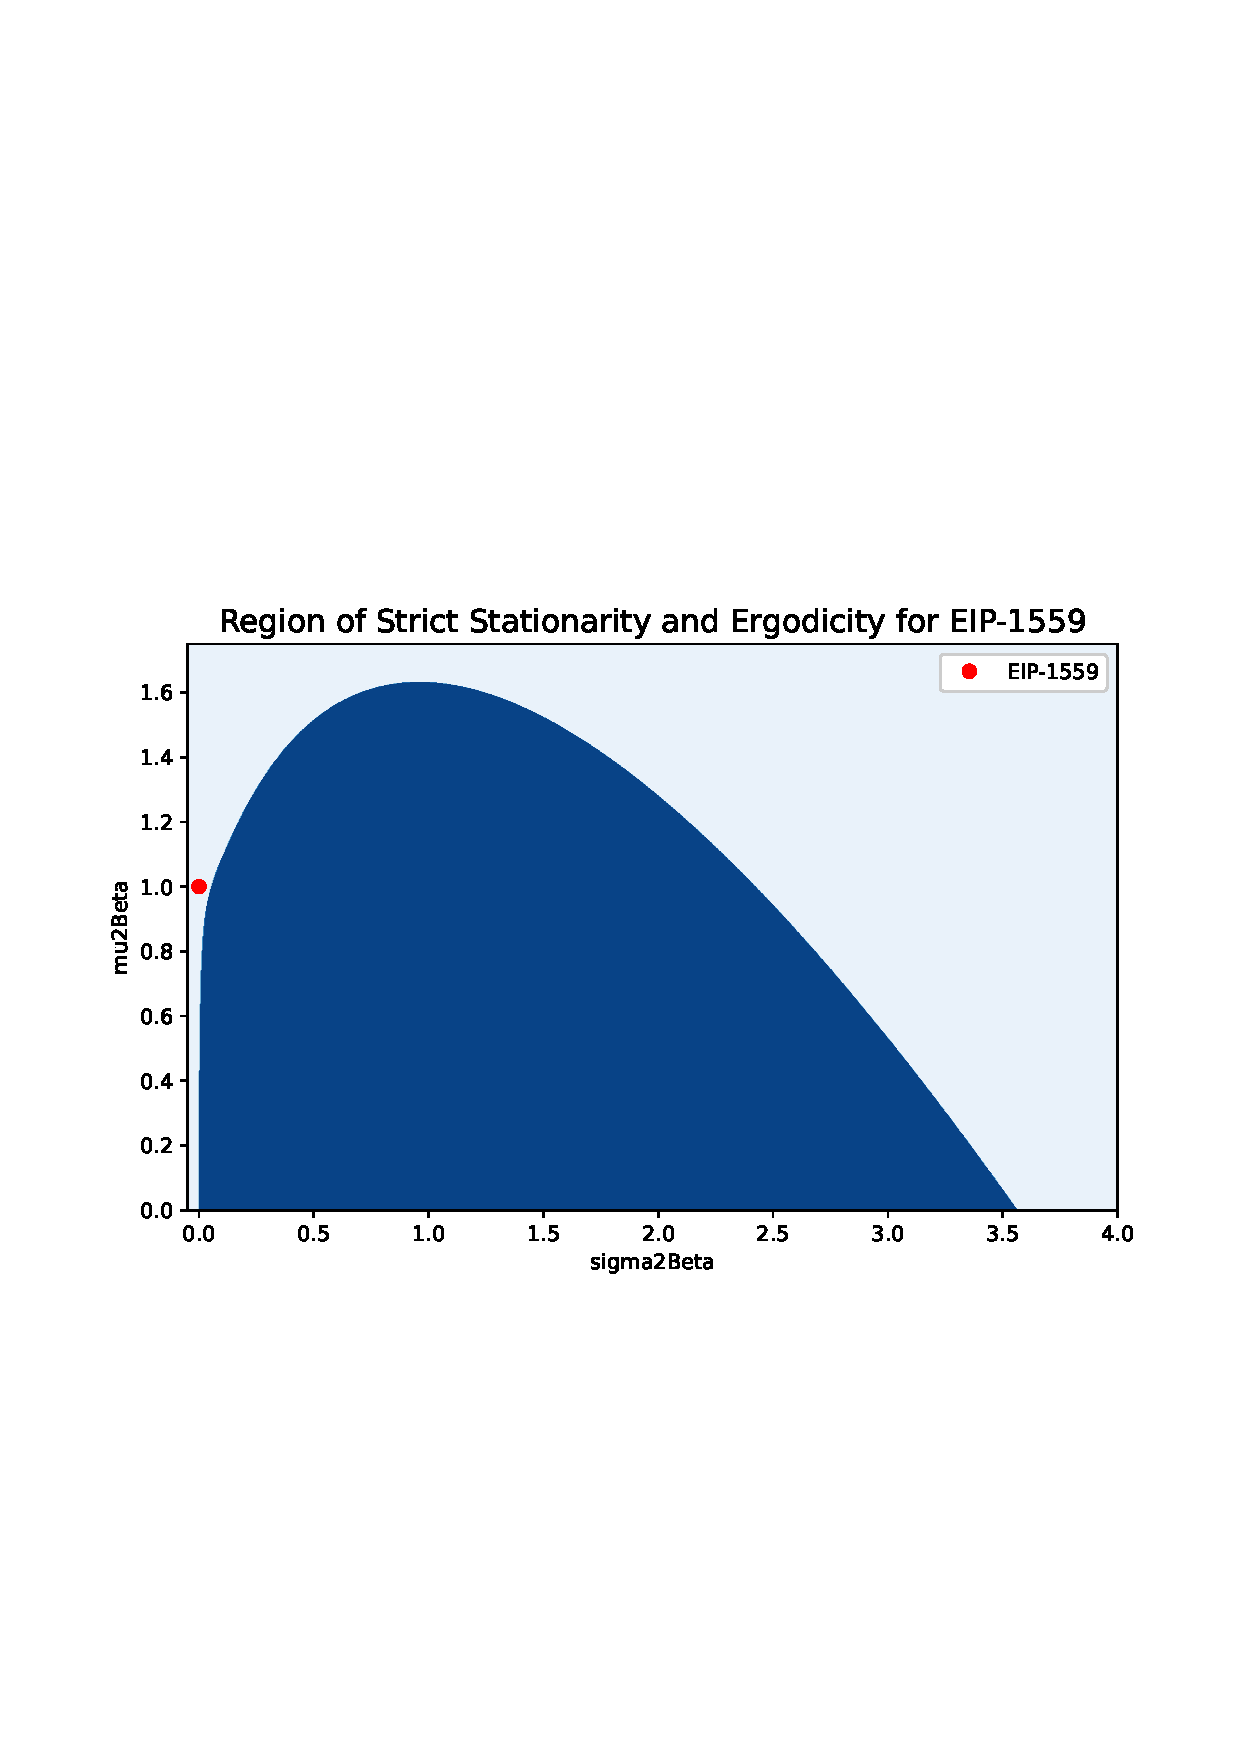
\includegraphics[width=3in]{img/strict_stationarity.png}
\caption{Strict stationarity} 
\label{fig:strict_stationarity}
\end{figure} 

\begin{figure}[h!]
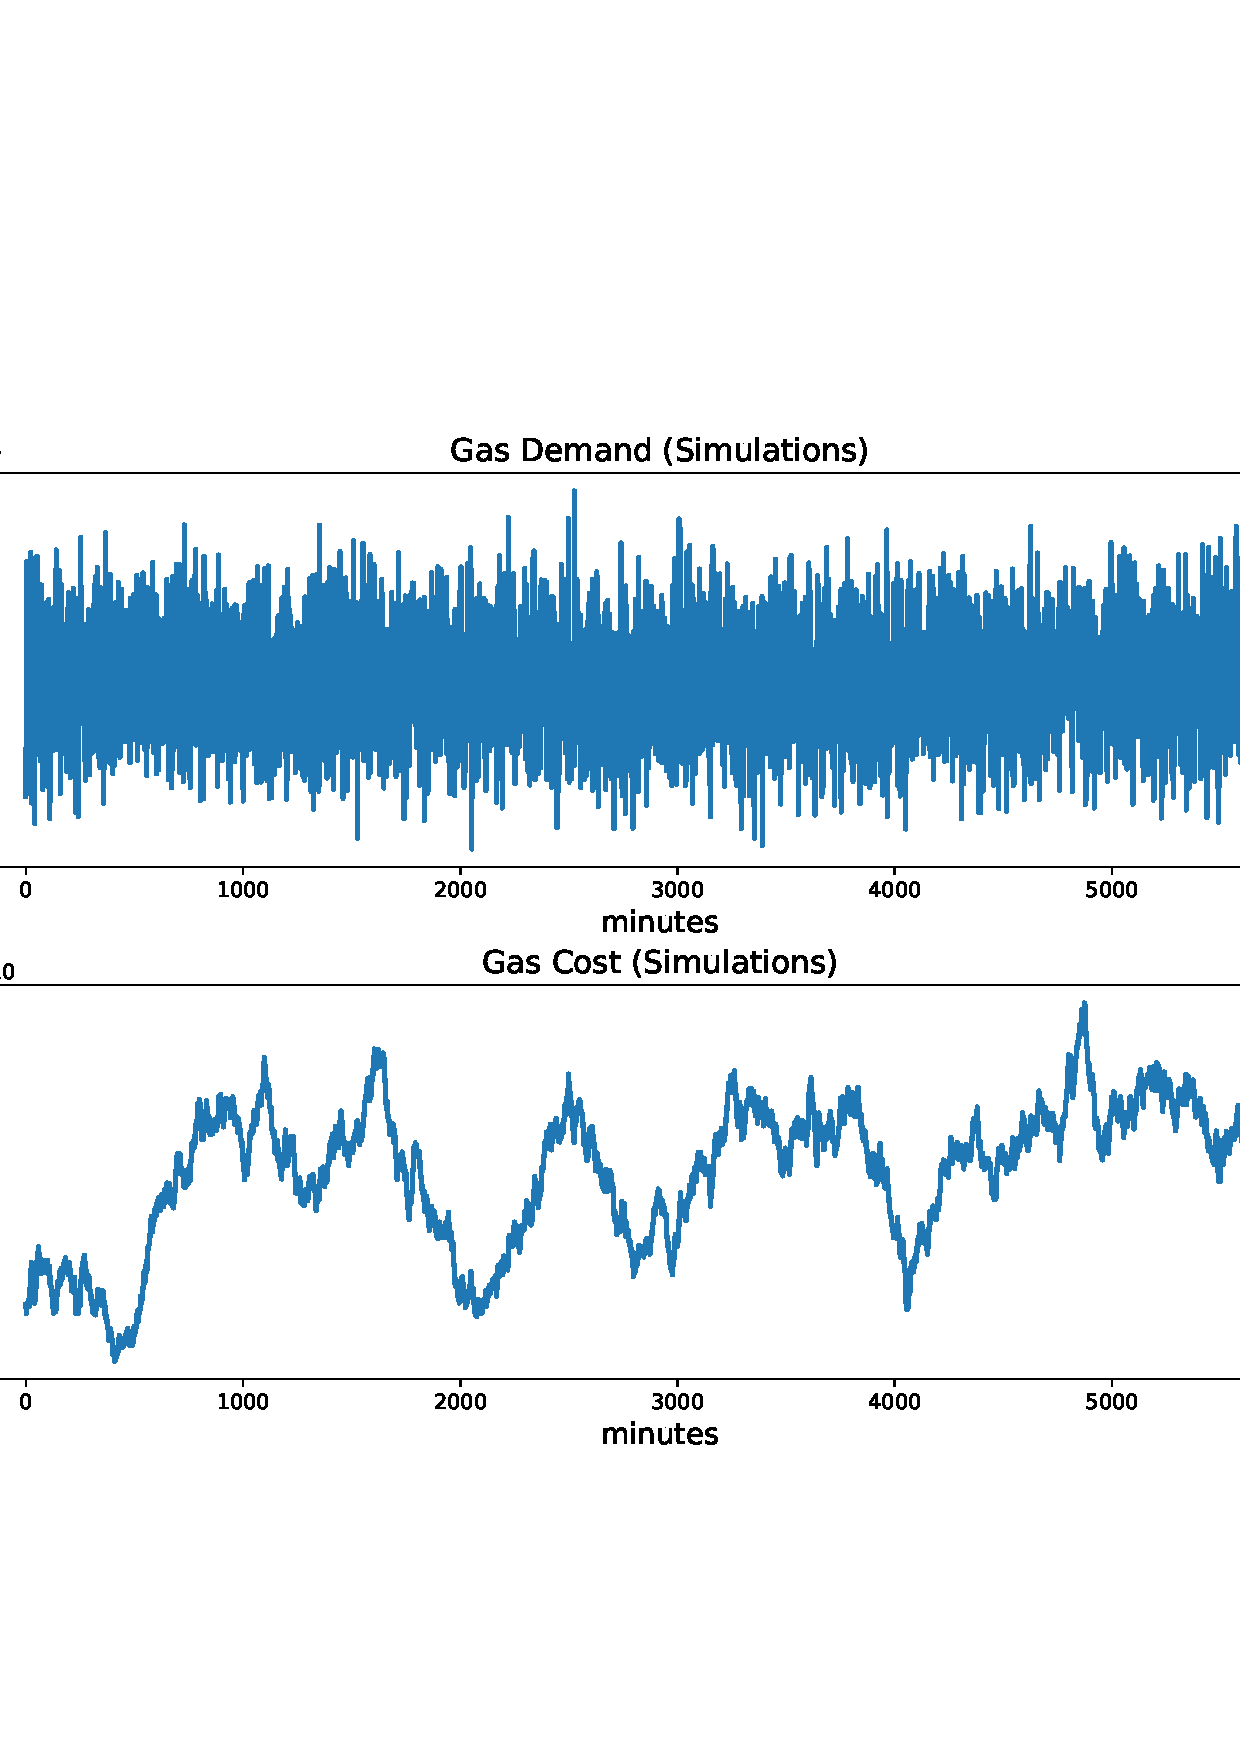
\includegraphics[width=3in]{img/gas.png}
\caption{Gas and demand simulations} 
\label{fig:gas}
\end{figure} 

\begin{figure}[h!]
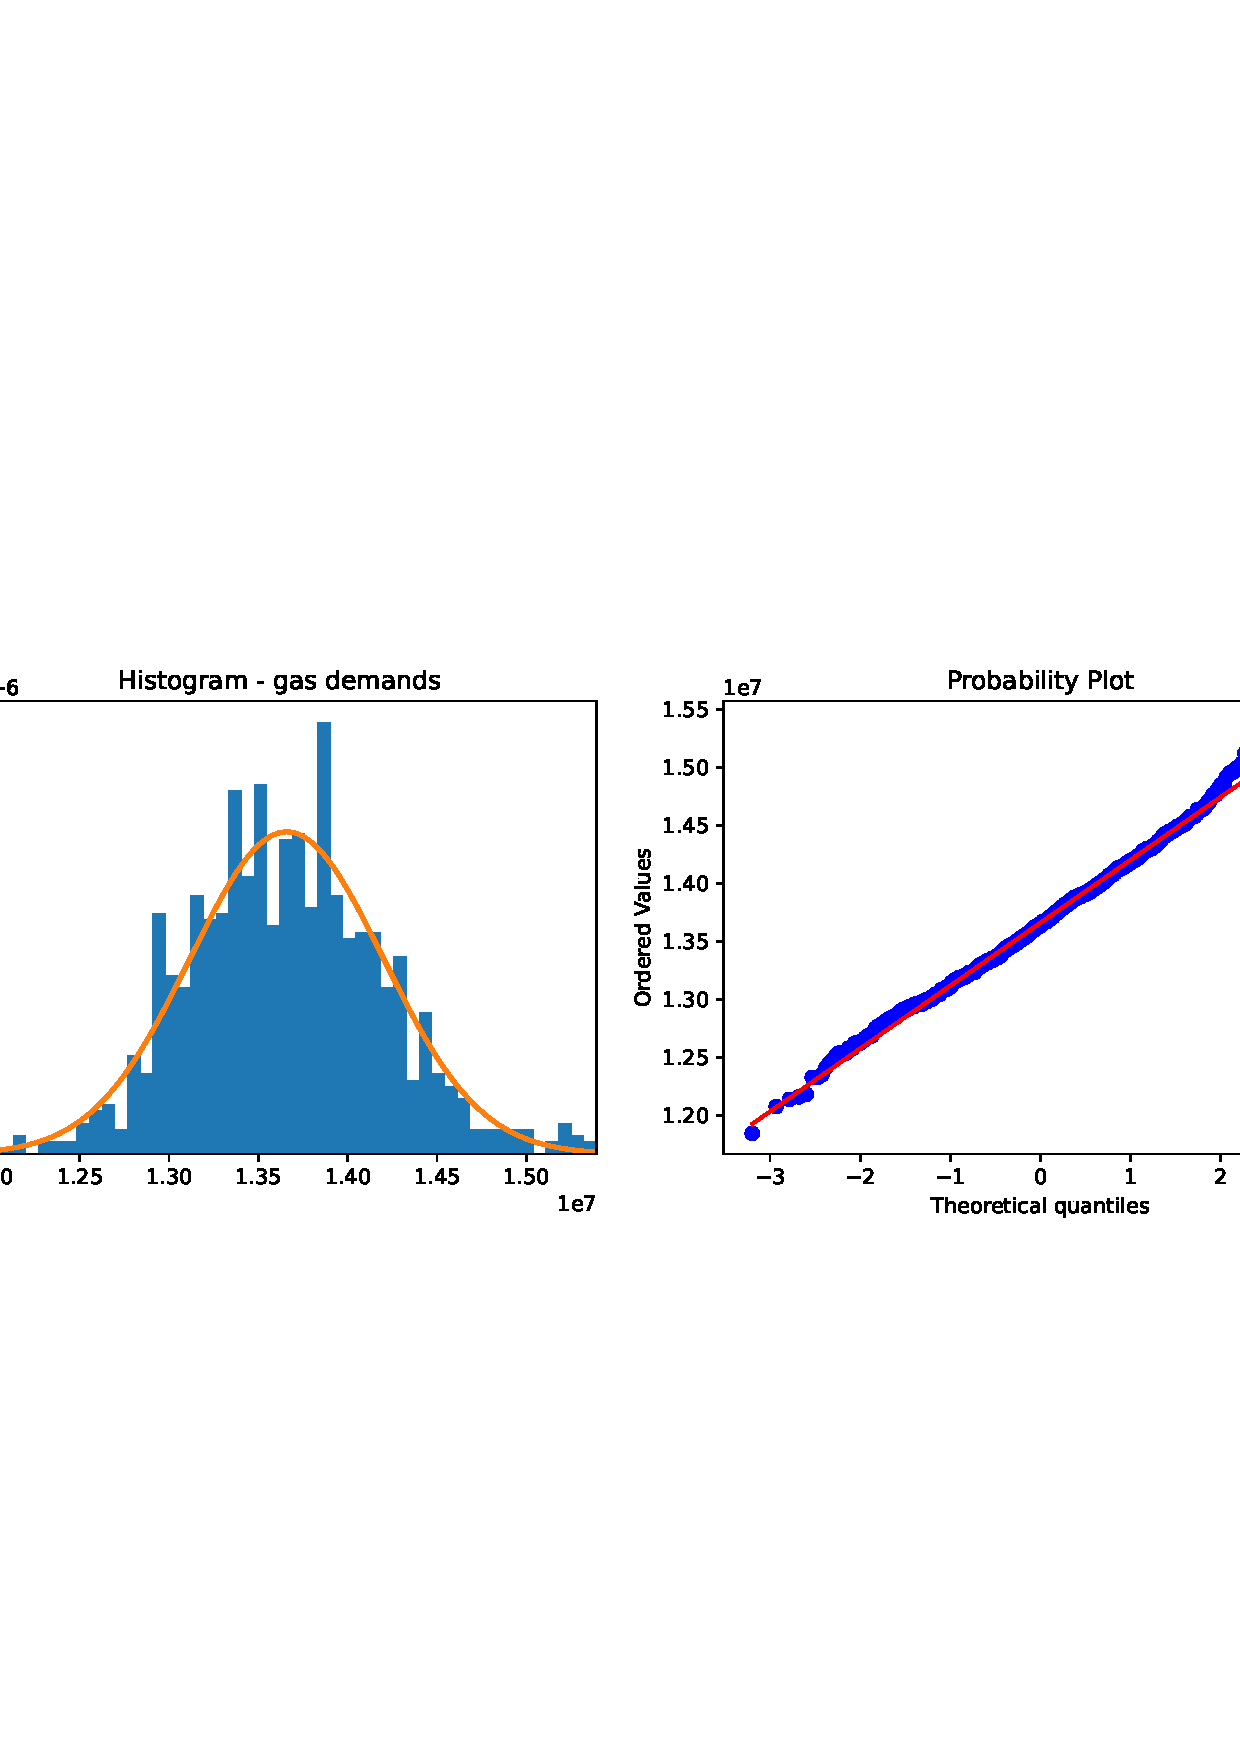
\includegraphics[width=3in]{img/gaussian_analysis.png}
\caption{Analysis of Normality of Gas Demands} 
\label{fig:gaussian_analysis}
\end{figure} 

\section{Conclusion}
\label{section:conclusion}
Praesent mauris. Fusce nec tellus sed augue semper porta. Mauris massa. Vestibulum lacinia arcu eget nulla. Class aptent taciti sociosqu ad litora torquent per conubia nostra, per inceptos himenaeos. Curabitur sodales ligula in libero. Sed dignissim lacinia nunc. Curabitur tortor. Pellentesque nibh. Aenean quam. In scelerisque sem at dolor. Maecenas mattis. Sed convallis tristique sem. 

\begin{thebibliography}{00}

\bibitem{Rou20} T. Roughgarden, \textit{Transaction Fee Mechanism Design for the Ethereum Blockchain: An Economic Analysis of EIP-1559}, Dec 2020. Accessed on: Apr 2021. [Online]. Available: https://arxiv.org/abs/2012.00854

\bibitem{Rou20} L. Trapani, \textit{Testing for Strict Stationarity in a Random Coefficient Autoregressive Model}, Jan 2019. Accessed on: Apr 2021. [Online]. Available: https://arxiv.org/abs/1901.01077

\bibitem{Cha89} C. Chatfield, \textit{The Analysis of Time Series: An Introduction. 4th Edition}, Chapman and Hall, New York, 1989

\bibitem{Nic82} D. Nicholls and B. Quinn , \textit{Random Coefficient Autoregressive Models: An Introduction}, Springer-Verlag, 1982

\bibitem{Wan03} Dazhe Wang, Frequentist and Bayesian Analysis of Random Coefficient Autoregressive Models, North Carolina State University PhD Dissertation, 2003

\bibitem{Mon21} B. Monnot, \textit{Agent-based Simulation Environment for EIP 1559}, Accessed on: Apr 2021.  [Online]. Available:  https://github.com/barnabemonnot/abm1559

\end{thebibliography}


\EOD

\end{document}
